\documentclass[12pt,a4paper]{article}
\usepackage[utf8]{inputenc}
\usepackage[czech]{babel}
\usepackage[T1]{fontenc}
\usepackage{amsmath}
\usepackage{amsfonts}
\usepackage{amssymb}
\usepackage{graphicx}
\usepackage{titlesec}
\usepackage[left=2cm,right=2cm,top=2cm,bottom=2cm]{geometry}
\usepackage{indentfirst}
\usepackage{listings}
\usepackage{color}
\usepackage{array}
\usepackage{csquotes}
\usepackage{subfig}

%Pravidlo pro řádkování
\renewcommand{\baselinestretch}{1.5}

%Pravidlo pro začínání kapitol na novém řádku
\let\oldsection\section
\renewcommand\section{\clearpage\oldsection}

%Formáty písem pro nadpisy (-změněno na bezpatkové \sffamily z původního \normalfont
\titleformat{\section}
{\sffamily\Large\bfseries}{\thesection}{1em}{}
\titleformat{\subsection}
{\sffamily\large\bfseries}{\thesubsection}{1em}{}
\titleformat{\subsubsection}
{\sffamily\normalsize\bfseries}{\thesubsubsection}{1em}{}

%Nastavení zvýrazňování kódu v \lslisting
\definecolor{mygreen}{rgb}{0,0.6,0}
\definecolor{mygray}{rgb}{0.5,0.5,0.5}
\lstset{commentstyle=\color{mygreen},keywordstyle=\color{blue},numberstyle=\tiny\color{mygray}}

\author{Jan Šmejkal}

\begin{document}

%-------------Úvodni strana---------------
\begin{titlepage}


\includegraphics[width=50mm]{img/FAV.jpg}
\\[160 pt]
\centerline{ \Huge \sc KIV/MKZ - Mobilní komunikace a zařízení}
\\[6 pt]
\centerline{ \LARGE \sc Semestrální práce}
\\[12 pt]
\centerline{ \large \sc Krátký proces}
\centerline{ \large \sc Android aplikace pro}


{
\vfill 
\parindent=0cm
\textbf{Jméno:} Štěpán Ševčík\\
\textbf{Osobní číslo:} A13B0443P\\
\textbf{E-mail:} kiwi@students.zcu.cz\\
\textbf{Datum:} {\large \today\par} %datum

}

\end{titlepage}

%------------------------------------------

%------------------Obsah-------------------
\newpage
\setcounter{page}{2}
\setcounter{tocdepth}{3}
\tableofcontents
%------------------------------------------

%--------------Text dokumentu--------------


\section{Zadání}
Vytvoření aplikace pro správu opakujících se procesů. Procesem se rozumí množina kroků výsledící v požadovaný stav. Procesy lze spouštět a u běhů procesů lze plnit jednotlivé kroky.

\section{Programátorská dokumentace}
\subsection{Analýza}
Ze zadání vyplývá požadavek na práci s proměnlivým počtem prvků různých typů. V práci k těmto prvkům budeme přistupovat jako k entitám. Ze zadání je dále zřejmé, že je potřeba definovat tyto entity:
\begin{itemize}
\item Proces (Process)
\item Krok procesu (ProcessStep)
\item Běh procesu (ProcessRun)
\item Krok běhu procesu (ProcessRunStep)
\end{itemize}

\subsection{Perzistence entit}
Entity na sebe vzájemně ukazují pomocí indexů a pro práci s nimi je vhodné použít databázi. Android poskytuje nativně ovladače pro práci s SQLite databázemi.

V aplikaci je kořenový prvek práce s databázemi třída \texttt{SQLiteHelper}. Tato třída poskytuje přístup ke službám, které zprostředkovávají konkrétní operace nad databází. Dále \texttt{SQLiteHelper} vytváří databázi, pokud neexistuje instance, pomocí SQL souboru obsahujícího definice tabulek.

Pro každý typ entity existuje v aplikaci služba pro práci s jejími instancemi. Tyto služby vycházejí ze společného generického základu, který poskytuje základní CRUD funkce.
Specifické služby potom obsahují pokročilejší funkce pro získávání instancí entit a dalších agregovaných informací.

Pro získávání instancí entit z výsledků dotazů do databáze je použit generický obal \texttt{ModelCursor}, který pomocí parseru mapuje řádky výsledku na instance entit.

\subsection{Uživatelské rozhraní}
Ve většině případů jsou použity pro zobrazování výsledků seznamy (\texttt{ListView}), které pomocí adaptérů a XML šablon definují způsob zobrazení entit.
Adaptéry těchto seznamů vycházejí z generického adaptéru \texttt{ModelListAdapter}, který sjednocuje běžně používané případy použití jako je například nastavení zobrazovaných položek z \texttt{ModelCursoru} nebo zpracování události kliknutí na řádek seznamu.

Události kliknutí jsou dále zpracovávány pomocí \texttt{EntityClickListener}.


\section{Uživatelská dokumentace}
Uživatelské rozhraní je pouze základní prototyp představující možné použití aplikace. Rozhraní obsahuje ostré hrany a nevypilované prvky a jeho použití je pouze na vlastní nebezpečí.

\begin{figure}[h]
	\centering
	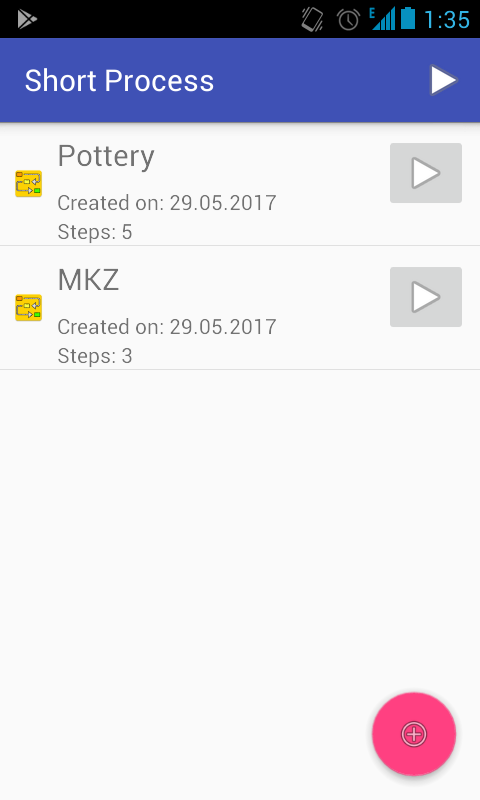
\includegraphics[width=0.4\linewidth]{img/fig_processList.png}
	\caption{Seznam procesů}
	\label{fig:processList}
\end{figure}

Po spuštění aplikace je uživatel přivítán pohledem Seznam procesů, viz Obrázek \ref{fig:processList}. Z tohoto pohledu může uživatel vytvářet nové procesy pomocí plovoucího akčního tlačítka nebo upravovat existující procesy klepnutím na jejich řádek.

Dále má uživatel možnost procesy spouštět klepnutím na příslušné tlačítko na řádku procesu, případně přejít na pohled běžících procesů.
\newpage
\begin{figure}
	\centering
	\subfloat[Editace procesu]{
		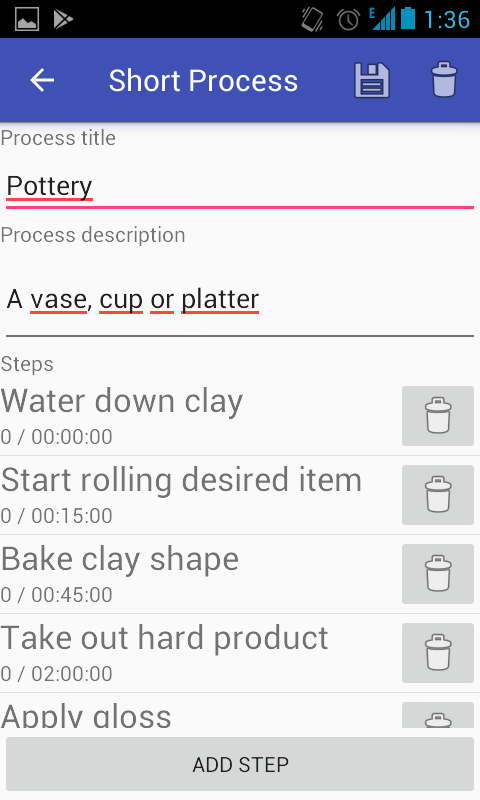
\includegraphics[width=0.4\linewidth]{img/fig_processEdit.png}
		\label{fig:processEdit}
	}
	\subfloat[Úprava kroku procesu]{
		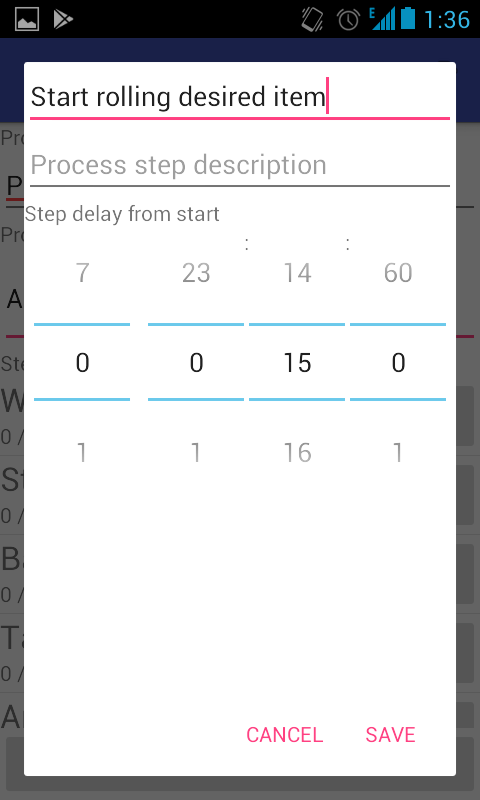
\includegraphics[width=0.4\linewidth]{img/fig_processStepEdit.png}
		\label{fig:processStepEdit}
	}
\caption{Úprava procesu}
\end{figure}
Editace nebo vytvoření procesu skrze pohled znázorněný Obrázkem \ref{fig:processEdit} umožňuje uživateli měnit název a popis procesu. Změny lze uložit pomocí tlačítka s ikonou diskety v nástrojové liště. Proces lze také smazat pomocí tlačítka v nástrojové liště s ikonou koše, po kterém se zobrazí ověřovací dialog.

Skrze tento pohled je také možné přidávat a mazat kroky procesu klepnutím na příslušné tlačítko nebo upravovat klepnutím na jejich řádek v seznamu. Úprava kroku probíhá v modálním okně znázorněného Obrázkem \ref{fig:processStepEdit}.

\newpage


V pohledu Seznam spuštěných procesů, který je znázorněn Obrázkem \ref{fig:processRuns}, je možné vidět souhrnné informace o běžících procesech anebo spuštěné procesy zastavit přislušným tlačítkem.
U spuštění procesů lze vybírat kroky, které jsou již splněny, pomocí modálního okna znázorněného Obrázkem \ref{fig:processRunSteps}.

\begin{figure}
	\centering
	\subfloat[Seznam spuštěných procesů]{
		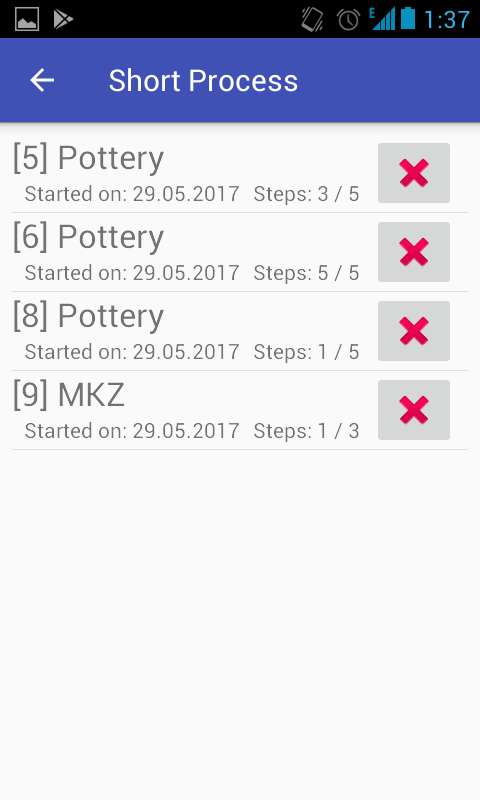
\includegraphics[width=0.4\linewidth]{img/fig_processRuns.png}
		\label{fig:processRuns}
	}
	\subfloat[Kroky spuštěného procesu]{
		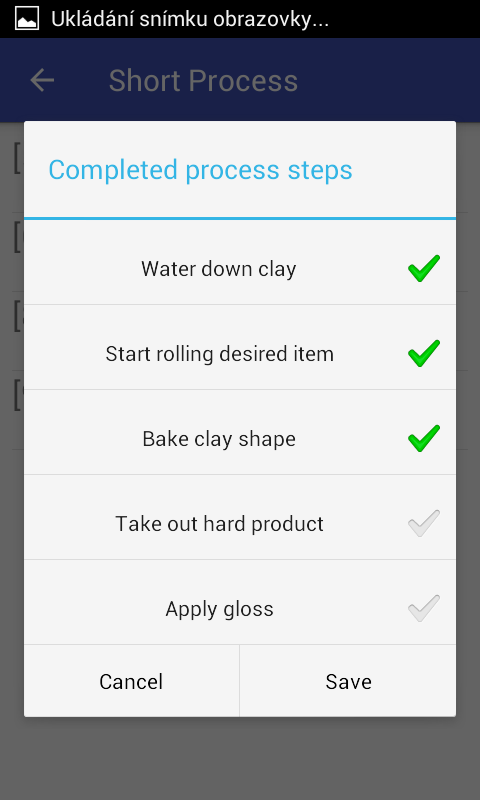
\includegraphics[width=0.4\linewidth]{img/fig_processRunSteps.png}
		\label{fig:processRunSteps}
	}
	\caption{Spuštěné procesy}
\end{figure}


\section{Vývoj}
Aplikace byla vyvíjena v prostředí Android Studio a testována na zařízení Huawei Ascend Y300 (Android 4.1.1, API level 16).

\subsection{Řešené problémy}
Při vývoji jsem narazil na překvapivé chování při konfiguraci minimální API úrovně 15 s prací s widgetem \texttt{NumberPicker}. Tento element nepodporuje nastavení minimální a maximální hodnoty v XML i přes to, že tyto hranice lze nastavit programově.

Podle odpovědi na StackOverflow jsem tento nedostatek vyřešil vytvořením odděděné třídy, která rozšiřuje funkčnost elementu \texttt{NumberPicker} právě o zpracování atributů \textit{min} a \textit{max}.

\section{Závěr}
V rámci této semestrální aplikace byla vytvořena aplikace pro správu procesů umožňující jejich vytváření, úpravy a spouštění.

Tuto aplikaci je možné rozšířit o zobrazování notifikací v časy odpovídající krokům spuštěných procesů a celkově o vylepšení životního cyklu procesu


%------------------------------------------

\end{document}
